\documentclass[a4paper,11pt,fleqn]{scrartcl}%fleqn pour aligner les equations à gauche
\usepackage{../../Styles/Exercice}

\newcommand{\chnum}{Chapitre 13}
\newcommand{\chtitle}{Mouvement et forces}
\newcommand{\dtype}{Exercices}

\begin{document}
\maketitle

\begin{multicols}{2}
\section{Connaître la direction et le sens de $\sum \vec{F}$}

Pour les tableaux ci-dessous, relier chaque schéma de $\Delta \vec{v}$ et $\vec{v}$ à la somme des forces $\sum \vec{F}$ qui lui correspond. Plusieurs schémas peuvent accepter la même réponse.
\begin{center}
\begin{tabular}{ccm{3cm}cc}
%\hline
A &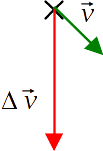
\includegraphics[scale=0.3]{Ressources/EX1_A.png} & &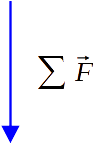
\includegraphics[scale=0.3]{Ressources/EX1_1.png}&1\\
%\hline
B &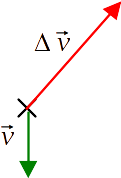
\includegraphics[scale=0.3]{Ressources/EX1_B.png} & &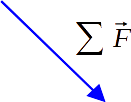
\includegraphics[scale=0.3]{Ressources/EX1_2.png}&2\\
%\hline
C &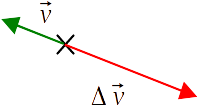
\includegraphics[scale=0.3]{Ressources/EX1_C.png} & &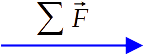
\includegraphics[scale=0.3]{Ressources/EX1_3.png}&3\\
%\hline
D &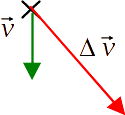
\includegraphics[scale=0.3]{Ressources/EX1_D.png} & &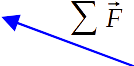
\includegraphics[scale=0.3]{Ressources/EX1_4.png}&4\\
%\hline
\end{tabular}
\end{center}

\section{Exploiter la somme des forces $\sum \vec{F}$}
1. Le mobile décrit une trajectoire circulaire uniforme  puis que les positions occupées par le mobile sont régulièrement espacées.\\
2. \begin{minipage}
{0.5\textwidth}
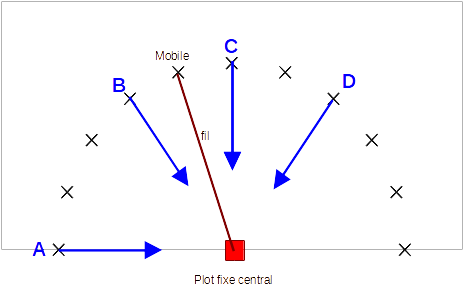
\includegraphics[scale=0.5]{Ressources/EX2.png}
\end{minipage}

\section{Connaître l'influence de la masse du système}
\begin{enumerate}
\item Le vecteur $\sum{\vec{F}}$ correspond à la somme des différents vecteurs forces. Ici puisque $\vec{P}$ et $\vec{R}$ sont opposés et de même norme, leur somme est nulle, ce qui nous donne donc : $$ \sum{\vec{F}} = \vec{P} - \vec{P} + \vec{f}= \vec{f} $$ La somme des forces est donc égale à la force de traction $\vec{f}$.
\item Puisque la somme des forces est égale à la masse multipliée par la variation de vitesse divisée par la durée, on peut en déduire que le vecteur variation de vitesse $\Delta \vec{v}$ a la même direction et le même sens que la force de traction $\vec{f}$.
\item En doublant la masse du système, on retrouve la relation : $$ \sum{\vec{F}}=2m \cdot \frac{\Delta \vec{v'}}{\Delta t} $$ Sachant que $\sum{\vec{F}}=m \cdot \frac{\Delta \vec{v}}{\Delta t}$, on peut en déduire que : $$ 2m \cdot \frac{\Delta \vec{v'}}{\Delta t} = m \cdot \frac{\Delta \vec{v}}{\Delta t} $$ $$ 2\Delta \vec{v'} = \Delta \vec{v} $$ $$ \Delta \vec{v'} = \frac{1}{2} \Delta \vec{v} $$ Le vecteur variation de vitesse du système de masse $2m$ est donc deux fois plus petit que celui du système de masse $m$.
\end{enumerate}

\section{Connaître l'influence de la masse (encore)}
Dans les deux situation schématisées ci-dessous, les deux systèmes, respectivement de masse $m$ et $m+m'$, sont soumis à la même somme des forces $\sum{\vec{F}}$. Les vecteurs variation de vitesse ont été représentés avec la même échelle.\\
\begin{center}
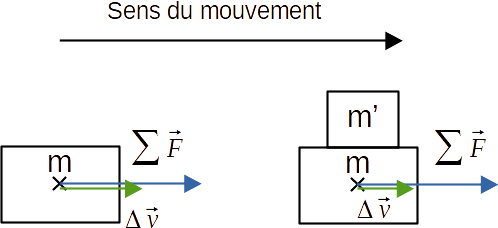
\includegraphics[width=.7\linewidth]{Ressources/EX4.png}\\
\end{center}
Justifier la différence entre les deux vecteurs variation de vitesse.
Sachant que les deux systèmes sont soumis à la même somme des forces, on peut en déduire que : $$ \sum{\vec{F}}=m \cdot \frac{\Delta \vec{v}}{\Delta t} = (m+m') \cdot \frac{\Delta \vec{v'}}{\Delta t} $$ 
On simplifie par $\Delta t$ : $$ m \cdot \Delta \vec{v} = (m+m') \cdot \Delta \vec{v'} $$ $$ \Delta \vec{v} = \frac{m+m'}{m} \cdot \Delta \vec{v'} $$ 
$$ \dfrac{\Delta \vec{v}}{\Delta \vec{v'}} = \frac{m+m'}{m} $$
Comme $m+m' > m$, on en déduit que $\Delta \vec{v} > \Delta \vec{v'}$. Le vecteur variation de vitesse du système de masse $m$ est plus grand que celui du système de masse $m+m'$ car la masse du second système est plus grande que celle du premier système.

\section{Thrust}
\begin{enumerate}
\item The speed variation vector has the same direction and the same sense as the motion of the aircraft, which is forward.
\item Since the aircraft is in accelerated rectilinear motion, the vector sum of the forces exerted on the aircraft has the same direction and the same sense as the speed variation vector, which is forward.
\item The thrust of the airplane has the same direction and the same sense as the vector sum of the forces exerted on the aircraft, which is forward.
\end{enumerate}

\section{Trampoline}

Sachant que l'athlète est soumis à la force de gravité, on peut en déduire que la somme des forces exercées sur lui est égale à son poids : $$ \sum{\vec{F}} = \vec{P} = m \cdot \vec{g} $$ Sachant que $\sum{\vec{F}}=m \cdot \frac{\Delta \vec{v}}{\Delta t}$, on peut en déduire que : $$ m \cdot \frac{\Delta \vec{v}}{\Delta t} = m \cdot \vec{g} $$ $$ \frac{\Delta \vec{v}}{\Delta t} = \vec{g} $$ $$ \Delta \vec{v} = \vec{g} \cdot \Delta t $$ Sachant que $\vec{g}$ a une norme de 9,81 m/s² et que $\Delta t$ est égal à 1,0 s, on trouve que : $$ |\Delta \vec{v}| = 9,81 m/s² \cdot 1,0 s = 9,81 m/s $$ La vitesse de l'athlète lorsqu'il retombe sur le trampoline est donc de 9,81 m/s.
\end{multicols}
\end{document}